% Options for packages loaded elsewhere
\PassOptionsToPackage{unicode}{hyperref}
\PassOptionsToPackage{hyphens}{url}
%
\documentclass[
]{article}
\usepackage{amsmath,amssymb}
\usepackage{lmodern}
\usepackage{iftex}
\ifPDFTeX
  \usepackage[T1]{fontenc}
  \usepackage[utf8]{inputenc}
  \usepackage{textcomp} % provide euro and other symbols
\else % if luatex or xetex
  \usepackage{unicode-math}
  \defaultfontfeatures{Scale=MatchLowercase}
  \defaultfontfeatures[\rmfamily]{Ligatures=TeX,Scale=1}
\fi
% Use upquote if available, for straight quotes in verbatim environments
\IfFileExists{upquote.sty}{\usepackage{upquote}}{}
\IfFileExists{microtype.sty}{% use microtype if available
  \usepackage[]{microtype}
  \UseMicrotypeSet[protrusion]{basicmath} % disable protrusion for tt fonts
}{}
\makeatletter
\@ifundefined{KOMAClassName}{% if non-KOMA class
  \IfFileExists{parskip.sty}{%
    \usepackage{parskip}
  }{% else
    \setlength{\parindent}{0pt}
    \setlength{\parskip}{6pt plus 2pt minus 1pt}}
}{% if KOMA class
  \KOMAoptions{parskip=half}}
\makeatother
\usepackage{xcolor}
\usepackage[margin=1in]{geometry}
\usepackage{color}
\usepackage{fancyvrb}
\newcommand{\VerbBar}{|}
\newcommand{\VERB}{\Verb[commandchars=\\\{\}]}
\DefineVerbatimEnvironment{Highlighting}{Verbatim}{commandchars=\\\{\}}
% Add ',fontsize=\small' for more characters per line
\usepackage{framed}
\definecolor{shadecolor}{RGB}{248,248,248}
\newenvironment{Shaded}{\begin{snugshade}}{\end{snugshade}}
\newcommand{\AlertTok}[1]{\textcolor[rgb]{0.94,0.16,0.16}{#1}}
\newcommand{\AnnotationTok}[1]{\textcolor[rgb]{0.56,0.35,0.01}{\textbf{\textit{#1}}}}
\newcommand{\AttributeTok}[1]{\textcolor[rgb]{0.77,0.63,0.00}{#1}}
\newcommand{\BaseNTok}[1]{\textcolor[rgb]{0.00,0.00,0.81}{#1}}
\newcommand{\BuiltInTok}[1]{#1}
\newcommand{\CharTok}[1]{\textcolor[rgb]{0.31,0.60,0.02}{#1}}
\newcommand{\CommentTok}[1]{\textcolor[rgb]{0.56,0.35,0.01}{\textit{#1}}}
\newcommand{\CommentVarTok}[1]{\textcolor[rgb]{0.56,0.35,0.01}{\textbf{\textit{#1}}}}
\newcommand{\ConstantTok}[1]{\textcolor[rgb]{0.00,0.00,0.00}{#1}}
\newcommand{\ControlFlowTok}[1]{\textcolor[rgb]{0.13,0.29,0.53}{\textbf{#1}}}
\newcommand{\DataTypeTok}[1]{\textcolor[rgb]{0.13,0.29,0.53}{#1}}
\newcommand{\DecValTok}[1]{\textcolor[rgb]{0.00,0.00,0.81}{#1}}
\newcommand{\DocumentationTok}[1]{\textcolor[rgb]{0.56,0.35,0.01}{\textbf{\textit{#1}}}}
\newcommand{\ErrorTok}[1]{\textcolor[rgb]{0.64,0.00,0.00}{\textbf{#1}}}
\newcommand{\ExtensionTok}[1]{#1}
\newcommand{\FloatTok}[1]{\textcolor[rgb]{0.00,0.00,0.81}{#1}}
\newcommand{\FunctionTok}[1]{\textcolor[rgb]{0.00,0.00,0.00}{#1}}
\newcommand{\ImportTok}[1]{#1}
\newcommand{\InformationTok}[1]{\textcolor[rgb]{0.56,0.35,0.01}{\textbf{\textit{#1}}}}
\newcommand{\KeywordTok}[1]{\textcolor[rgb]{0.13,0.29,0.53}{\textbf{#1}}}
\newcommand{\NormalTok}[1]{#1}
\newcommand{\OperatorTok}[1]{\textcolor[rgb]{0.81,0.36,0.00}{\textbf{#1}}}
\newcommand{\OtherTok}[1]{\textcolor[rgb]{0.56,0.35,0.01}{#1}}
\newcommand{\PreprocessorTok}[1]{\textcolor[rgb]{0.56,0.35,0.01}{\textit{#1}}}
\newcommand{\RegionMarkerTok}[1]{#1}
\newcommand{\SpecialCharTok}[1]{\textcolor[rgb]{0.00,0.00,0.00}{#1}}
\newcommand{\SpecialStringTok}[1]{\textcolor[rgb]{0.31,0.60,0.02}{#1}}
\newcommand{\StringTok}[1]{\textcolor[rgb]{0.31,0.60,0.02}{#1}}
\newcommand{\VariableTok}[1]{\textcolor[rgb]{0.00,0.00,0.00}{#1}}
\newcommand{\VerbatimStringTok}[1]{\textcolor[rgb]{0.31,0.60,0.02}{#1}}
\newcommand{\WarningTok}[1]{\textcolor[rgb]{0.56,0.35,0.01}{\textbf{\textit{#1}}}}
\usepackage{graphicx}
\makeatletter
\def\maxwidth{\ifdim\Gin@nat@width>\linewidth\linewidth\else\Gin@nat@width\fi}
\def\maxheight{\ifdim\Gin@nat@height>\textheight\textheight\else\Gin@nat@height\fi}
\makeatother
% Scale images if necessary, so that they will not overflow the page
% margins by default, and it is still possible to overwrite the defaults
% using explicit options in \includegraphics[width, height, ...]{}
\setkeys{Gin}{width=\maxwidth,height=\maxheight,keepaspectratio}
% Set default figure placement to htbp
\makeatletter
\def\fps@figure{htbp}
\makeatother
\setlength{\emergencystretch}{3em} % prevent overfull lines
\providecommand{\tightlist}{%
  \setlength{\itemsep}{0pt}\setlength{\parskip}{0pt}}
\setcounter{secnumdepth}{-\maxdimen} % remove section numbering
\ifLuaTeX
  \usepackage{selnolig}  % disable illegal ligatures
\fi
\IfFileExists{bookmark.sty}{\usepackage{bookmark}}{\usepackage{hyperref}}
\IfFileExists{xurl.sty}{\usepackage{xurl}}{} % add URL line breaks if available
\urlstyle{same} % disable monospaced font for URLs
\hypersetup{
  pdftitle={HW 3: Random Number STreams},
  pdfauthor={Sokona Mangane},
  hidelinks,
  pdfcreator={LaTeX via pandoc}}

\title{HW 3: Random Number STreams}
\author{Sokona Mangane}
\date{2023-02-04}

\begin{document}
\maketitle

\hypertarget{dcs-307---hw-3}{%
\section{DCS 307 - HW 3}\label{dcs-307---hw-3}}

\begin{Shaded}
\begin{Highlighting}[]
\CommentTok{\#tinytex::install\_tinytex(), to knit as a PDF}
\FunctionTok{library}\NormalTok{(simEd)}
\end{Highlighting}
\end{Shaded}

\hypertarget{question-1-what-are-the-first-ten-service-times-from-the-first-run}{%
\subsection{Question 1: What are the first ten service times from the
first
run?}\label{question-1-what-are-the-first-ten-service-times-from-the-first-run}}

These are the first 10 service times from the second run: 0.6906071,
0.2777054, 0.1499705, 0.6604378, 0.5704503, 0.1073709, 0.3050448,
0.640531, 1.4994352, 0.2054382

\hypertarget{question-2-what-are-the-first-ten-service-times-from-the-second-run}{%
\subsection{Question 2: What are the first ten service times from the
second
run?}\label{question-2-what-are-the-first-ten-service-times-from-the-second-run}}

These are the first 10 service times from the second run: 0.6906071,
0.2777054, 0.1499705, 0.6604378, 0.388547, 2.7028233, 1.4994352,
0.8472361, 1.8154944, 2.7168156

\hypertarget{question-3-for-what-customer-and-what-are-the-different-values-where-the-first-service-time-diverges-between-the-two-runs}{%
\subsection{Question 3: For what customer, and what are the different
values, where the first service time diverges between the two
runs?}\label{question-3-for-what-customer-and-what-are-the-different-values-where-the-first-service-time-diverges-between-the-two-runs}}

The service time for the 5th customer is where we see different values,
where for the first run, we get a service time of 0.5704503 and for the
second run, we get a service time of 0.388547

\hypertarget{question-4-in-the-first-run-how-many-arrivals-occur-after-the-fourth-arrival-but-before-that-fourth-customer-completes-service}{%
\subsection{Question 4: In the first run, how many arrivals occur after
the fourth arrival, but before that fourth customer completes
service?}\label{question-4-in-the-first-run-how-many-arrivals-occur-after-the-fourth-arrival-but-before-that-fourth-customer-completes-service}}

\begin{Shaded}
\begin{Highlighting}[]
\FunctionTok{par}\NormalTok{(}\AttributeTok{mfrow =} \FunctionTok{c}\NormalTok{(}\DecValTok{2}\NormalTok{,}\DecValTok{1}\NormalTok{))}

\NormalTok{indices }\OtherTok{=} \FunctionTok{seq\_along}\NormalTok{(output1}\SpecialCharTok{$}\NormalTok{numInSystemT[output1}\SpecialCharTok{$}\NormalTok{numInSystemT }\SpecialCharTok{\textless{}=} \DecValTok{5}\NormalTok{])}
\FunctionTok{plot}\NormalTok{(output1}\SpecialCharTok{$}\NormalTok{numInSystemT[indices], output1}\SpecialCharTok{$}\NormalTok{numInSystemN[indices], }\AttributeTok{type =} \StringTok{"s"}\NormalTok{, }\AttributeTok{xlim =} \FunctionTok{c}\NormalTok{(}\DecValTok{0}\NormalTok{,}\DecValTok{5}\NormalTok{), }\AttributeTok{bty =} \StringTok{"n"}\NormalTok{, }\AttributeTok{las =} \DecValTok{1}\NormalTok{)}
\FunctionTok{abline}\NormalTok{(}\AttributeTok{v =} \FloatTok{4.562}\NormalTok{, }\AttributeTok{col =} \StringTok{"red"}\NormalTok{, }\AttributeTok{lwd=}\DecValTok{3}\NormalTok{, }\AttributeTok{lty=}\DecValTok{2}\NormalTok{)}

\NormalTok{indices }\OtherTok{=} \FunctionTok{seq\_along}\NormalTok{(output2}\SpecialCharTok{$}\NormalTok{numInSystemT[output2}\SpecialCharTok{$}\NormalTok{numInSystemT }\SpecialCharTok{\textless{}=} \DecValTok{5}\NormalTok{])}
\FunctionTok{plot}\NormalTok{(output2}\SpecialCharTok{$}\NormalTok{numInSystemT[indices], output2}\SpecialCharTok{$}\NormalTok{numInSystemN[indices], }\AttributeTok{type =} \StringTok{"s"}\NormalTok{, }\AttributeTok{xlim =} \FunctionTok{c}\NormalTok{(}\DecValTok{0}\NormalTok{,}\DecValTok{5}\NormalTok{), }\AttributeTok{bty =} \StringTok{"n"}\NormalTok{, }\AttributeTok{las =} \DecValTok{1}\NormalTok{)}
\FunctionTok{abline}\NormalTok{(}\AttributeTok{v =} \FloatTok{4.2}\NormalTok{, }\AttributeTok{col =} \StringTok{"red"}\NormalTok{, }\AttributeTok{lwd=}\DecValTok{3}\NormalTok{, }\AttributeTok{lty=}\DecValTok{2}\NormalTok{)}
\end{Highlighting}
\end{Shaded}

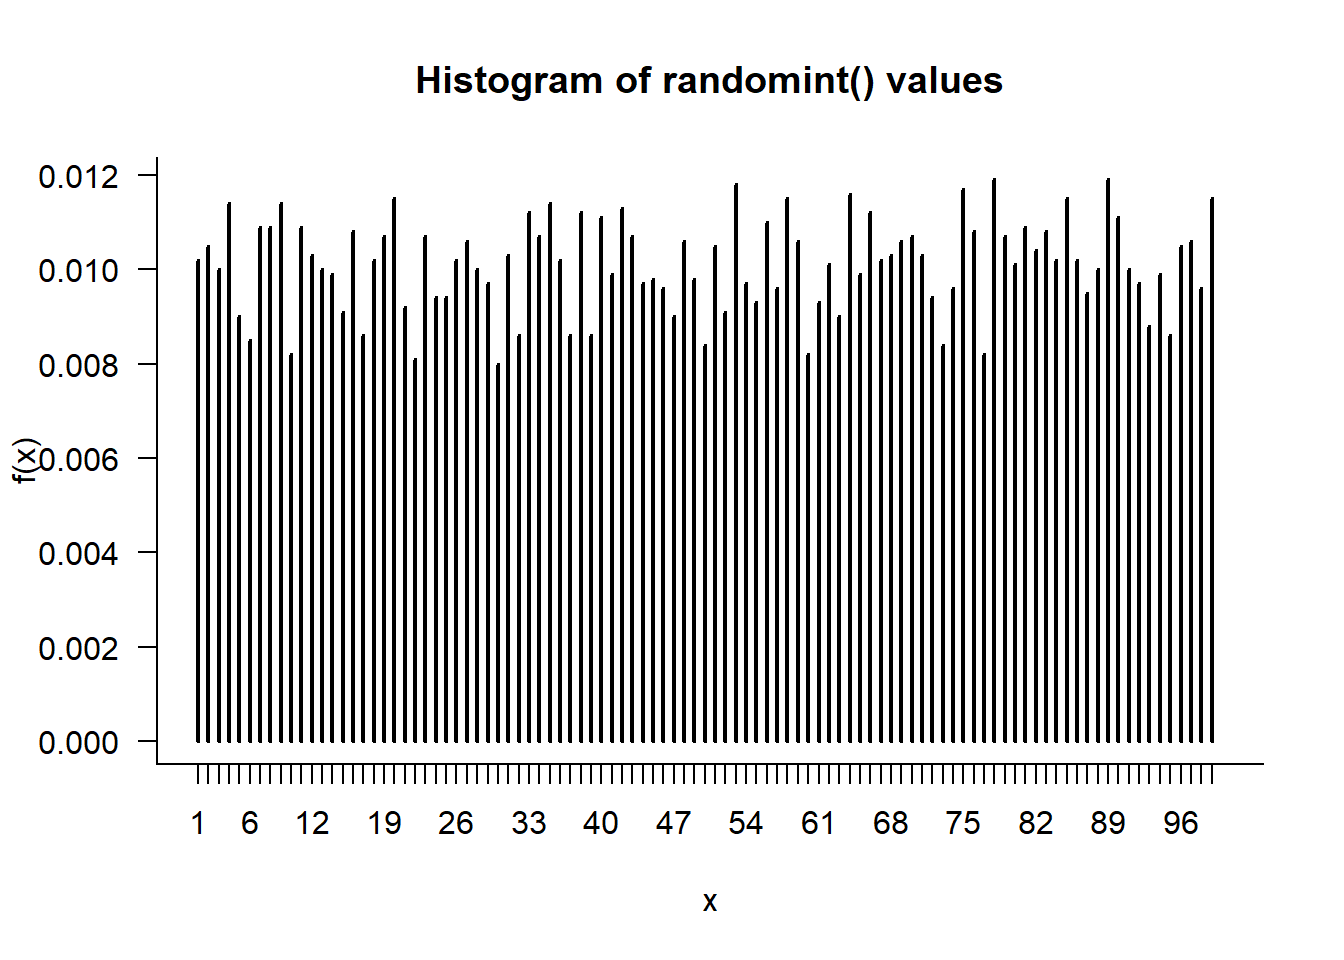
\includegraphics{Hw3_files/figure-latex/unnamed-chunk-1-1.pdf}

2 arrivals

\hypertarget{question-5-in-the-second-run-how-many-arrivals-occur-after-the-fourth-arrival-but-before-that-fourth-customer-completes-service}{%
\subsection{Question 5: In the second run, how many arrivals occur after
the fourth arrival, but before that fourth customer completes
service?}\label{question-5-in-the-second-run-how-many-arrivals-occur-after-the-fourth-arrival-but-before-that-fourth-customer-completes-service}}

3 arrivals

\hypertarget{question-6-what-are-the-arrival-times-rate-1-generated-using-rexp-no-streams}{%
\subsection{Question 6: What are the arrival times (rate = 1) generated
using rexp (no
streams)?}\label{question-6-what-are-the-arrival-times-rate-1-generated-using-rexp-no-streams}}

\begin{Shaded}
\begin{Highlighting}[]
\FunctionTok{set.seed}\NormalTok{(}\DecValTok{8675309}\NormalTok{)}
\FunctionTok{rexp}\NormalTok{(}\DecValTok{1}\NormalTok{,}\AttributeTok{rate =} \DecValTok{1}\NormalTok{)}
\end{Highlighting}
\end{Shaded}

\begin{verbatim}
## [1] 1.662163
\end{verbatim}

\begin{Shaded}
\begin{Highlighting}[]
\FunctionTok{rexp}\NormalTok{(}\DecValTok{1}\NormalTok{,}\AttributeTok{rate =} \DecValTok{1}\NormalTok{)}
\end{Highlighting}
\end{Shaded}

\begin{verbatim}
## [1] 1.223265
\end{verbatim}

\begin{Shaded}
\begin{Highlighting}[]
\FunctionTok{rexp}\NormalTok{(}\DecValTok{1}\NormalTok{,}\AttributeTok{rate =} \DecValTok{1}\NormalTok{)}
\end{Highlighting}
\end{Shaded}

\begin{verbatim}
## [1] 0.7673412
\end{verbatim}

\hypertarget{what-are-the-service-times-rate-109-generated-using-rexp-no-streams}{%
\subsection{What are the service times (rate = 10/9) generated using
rexp (no
streams)?}\label{what-are-the-service-times-rate-109-generated-using-rexp-no-streams}}

\begin{Shaded}
\begin{Highlighting}[]
\FunctionTok{set.seed}\NormalTok{(}\DecValTok{8675309}\NormalTok{)}
\FunctionTok{rexp}\NormalTok{(}\DecValTok{1}\NormalTok{,}\AttributeTok{rate =} \DecValTok{10}\SpecialCharTok{/}\DecValTok{9}\NormalTok{)}
\end{Highlighting}
\end{Shaded}

\begin{verbatim}
## [1] 1.495947
\end{verbatim}

\begin{Shaded}
\begin{Highlighting}[]
\FunctionTok{rexp}\NormalTok{(}\DecValTok{1}\NormalTok{,}\AttributeTok{rate =} \DecValTok{10}\SpecialCharTok{/}\DecValTok{9}\NormalTok{)}
\end{Highlighting}
\end{Shaded}

\begin{verbatim}
## [1] 1.100939
\end{verbatim}

\begin{Shaded}
\begin{Highlighting}[]
\FunctionTok{rexp}\NormalTok{(}\DecValTok{1}\NormalTok{,}\AttributeTok{rate =} \DecValTok{10}\SpecialCharTok{/}\DecValTok{9}\NormalTok{)}
\end{Highlighting}
\end{Shaded}

\begin{verbatim}
## [1] 0.6906071
\end{verbatim}

\hypertarget{now-what-are-the-arrival-times-rate-1-generated-using-rexp-no-streams}{%
\subsection{Now what are the arrival times (rate = 1) generated using
rexp (no
streams)?}\label{now-what-are-the-arrival-times-rate-1-generated-using-rexp-no-streams}}

\begin{Shaded}
\begin{Highlighting}[]
\FunctionTok{set.seed}\NormalTok{(}\DecValTok{8675309}\NormalTok{)}
\NormalTok{a1 }\OtherTok{=} \FunctionTok{rexp}\NormalTok{(}\DecValTok{1}\NormalTok{,}\AttributeTok{rate =} \DecValTok{1}\NormalTok{)}
\NormalTok{s1 }\OtherTok{=} \FunctionTok{rexp}\NormalTok{(}\DecValTok{1}\NormalTok{,}\AttributeTok{rate =} \DecValTok{10}\SpecialCharTok{/}\DecValTok{9}\NormalTok{)}
\NormalTok{a2 }\OtherTok{=} \FunctionTok{rexp}\NormalTok{(}\DecValTok{1}\NormalTok{,}\AttributeTok{rate =} \DecValTok{1}\NormalTok{)}
\NormalTok{s2 }\OtherTok{=} \FunctionTok{rexp}\NormalTok{(}\DecValTok{1}\NormalTok{,}\AttributeTok{rate =} \DecValTok{10}\SpecialCharTok{/}\DecValTok{9}\NormalTok{)}
\NormalTok{a3 }\OtherTok{=} \FunctionTok{rexp}\NormalTok{(}\DecValTok{1}\NormalTok{,}\AttributeTok{rate =} \DecValTok{1}\NormalTok{)}
\NormalTok{s3 }\OtherTok{=} \FunctionTok{rexp}\NormalTok{(}\DecValTok{1}\NormalTok{,}\AttributeTok{rate =} \DecValTok{10}\SpecialCharTok{/}\DecValTok{9}\NormalTok{)}
\end{Highlighting}
\end{Shaded}

The arrival times generated using rexp is 1.6621634, 0.7673412, and
0.3085615.

\hypertarget{now-what-are-the-service-times-rate-109-generated-using-rexp-no-streams}{%
\subsection{Now what are the service times (rate = 10/9) generated using
rexp (no
streams)?}\label{now-what-are-the-service-times-rate-109-generated-using-rexp-no-streams}}

The service times generated using rexp is 1.1009387, 0.3114826, and
0.6088186.

\hypertarget{what-are-the-arrival-times-rate-1-generated-using-vexp-with-streams}{%
\subsection{What are the arrival times (rate = 1) generated using vexp
(with
streams)?}\label{what-are-the-arrival-times-rate-1-generated-using-vexp-with-streams}}

\begin{Shaded}
\begin{Highlighting}[]
\FunctionTok{set.seed}\NormalTok{(}\DecValTok{8675309}\NormalTok{)}
\FunctionTok{vexp}\NormalTok{(}\DecValTok{1}\NormalTok{,}\AttributeTok{rate =} \DecValTok{1}\NormalTok{, }\AttributeTok{stream =} \DecValTok{1}\NormalTok{)}
\end{Highlighting}
\end{Shaded}

\begin{verbatim}
## [1] 0.2334595
\end{verbatim}

\begin{Shaded}
\begin{Highlighting}[]
\FunctionTok{vexp}\NormalTok{(}\DecValTok{1}\NormalTok{,}\AttributeTok{rate =} \DecValTok{1}\NormalTok{, }\AttributeTok{stream =} \DecValTok{1}\NormalTok{)}
\end{Highlighting}
\end{Shaded}

\begin{verbatim}
## [1] 1.07828
\end{verbatim}

\begin{Shaded}
\begin{Highlighting}[]
\FunctionTok{vexp}\NormalTok{(}\DecValTok{1}\NormalTok{,}\AttributeTok{rate =} \DecValTok{1}\NormalTok{, }\AttributeTok{stream =} \DecValTok{1}\NormalTok{)}
\end{Highlighting}
\end{Shaded}

\begin{verbatim}
## [1] 0.7855611
\end{verbatim}

\hypertarget{what-are-the-service-times-rate-109-generated-using-vexp-with-streams}{%
\subsection{What are the service times (rate = 10/9) generated using
vexp (with
streams)?}\label{what-are-the-service-times-rate-109-generated-using-vexp-with-streams}}

\begin{Shaded}
\begin{Highlighting}[]
\FunctionTok{set.seed}\NormalTok{(}\DecValTok{8675309}\NormalTok{)}
\FunctionTok{vexp}\NormalTok{(}\DecValTok{1}\NormalTok{,}\AttributeTok{rate =} \DecValTok{10}\SpecialCharTok{/}\DecValTok{9}\NormalTok{, }\AttributeTok{stream =} \DecValTok{2}\NormalTok{)}
\end{Highlighting}
\end{Shaded}

\begin{verbatim}
## [1] 0.0305915
\end{verbatim}

\begin{Shaded}
\begin{Highlighting}[]
\FunctionTok{vexp}\NormalTok{(}\DecValTok{1}\NormalTok{,}\AttributeTok{rate =} \DecValTok{10}\SpecialCharTok{/}\DecValTok{9}\NormalTok{, }\AttributeTok{stream =} \DecValTok{2}\NormalTok{)}
\end{Highlighting}
\end{Shaded}

\begin{verbatim}
## [1] 0.1224158
\end{verbatim}

\begin{Shaded}
\begin{Highlighting}[]
\FunctionTok{vexp}\NormalTok{(}\DecValTok{1}\NormalTok{,}\AttributeTok{rate =} \DecValTok{10}\SpecialCharTok{/}\DecValTok{9}\NormalTok{, }\AttributeTok{stream =} \DecValTok{2}\NormalTok{)}
\end{Highlighting}
\end{Shaded}

\begin{verbatim}
## [1] 1.42499
\end{verbatim}

\hypertarget{now-what-are-the-arrival-times-rate-1-generated-using-vexp-with-streams}{%
\subsection{Now what are the arrival times (rate = 1) generated using
vexp (with
streams)?}\label{now-what-are-the-arrival-times-rate-1-generated-using-vexp-with-streams}}

\begin{Shaded}
\begin{Highlighting}[]
\FunctionTok{set.seed}\NormalTok{(}\DecValTok{8675309}\NormalTok{)}
\NormalTok{a4 }\OtherTok{=} \FunctionTok{vexp}\NormalTok{(}\DecValTok{1}\NormalTok{,}\AttributeTok{rate =} \DecValTok{1}\NormalTok{, }\AttributeTok{stream =} \DecValTok{1}\NormalTok{)}
\NormalTok{s4 }\OtherTok{=} \FunctionTok{vexp}\NormalTok{(}\DecValTok{1}\NormalTok{,}\AttributeTok{rate =} \DecValTok{10}\SpecialCharTok{/}\DecValTok{9}\NormalTok{, }\AttributeTok{stream =} \DecValTok{2}\NormalTok{)}
\NormalTok{a5 }\OtherTok{=} \FunctionTok{vexp}\NormalTok{(}\DecValTok{1}\NormalTok{,}\AttributeTok{rate =} \DecValTok{1}\NormalTok{, }\AttributeTok{stream =} \DecValTok{1}\NormalTok{)}
\NormalTok{s5 }\OtherTok{=} \FunctionTok{vexp}\NormalTok{(}\DecValTok{1}\NormalTok{,}\AttributeTok{rate =} \DecValTok{10}\SpecialCharTok{/}\DecValTok{9}\NormalTok{, }\AttributeTok{stream =} \DecValTok{2}\NormalTok{)}
\NormalTok{a6 }\OtherTok{=} \FunctionTok{vexp}\NormalTok{(}\DecValTok{1}\NormalTok{,}\AttributeTok{rate =} \DecValTok{1}\NormalTok{, }\AttributeTok{stream =} \DecValTok{1}\NormalTok{)}
\NormalTok{s6 }\OtherTok{=} \FunctionTok{vexp}\NormalTok{(}\DecValTok{1}\NormalTok{,}\AttributeTok{rate =} \DecValTok{10}\SpecialCharTok{/}\DecValTok{9}\NormalTok{, }\AttributeTok{stream =} \DecValTok{2}\NormalTok{)}
\end{Highlighting}
\end{Shaded}

The arrival times generated using vexp is 0.2334595, 1.0782802, and
0.7855611.

\hypertarget{now-what-are-the-service-times-rate-109-generated-using-vexp-with-streams}{%
\subsection{Now what are the service times (rate = 10/9) generated using
vexp (with
streams)?}\label{now-what-are-the-service-times-rate-109-generated-using-vexp-with-streams}}

The arrival times generated using vexp is 0.0305915, 0.1224158, and
1.4249899.

\hypertarget{what-is-the-result-of-the-following}{%
\subsection{What is the result of the
following?}\label{what-is-the-result-of-the-following}}

\begin{Shaded}
\begin{Highlighting}[]
\NormalTok{myArr1ws }\OtherTok{\textless{}{-}} \ControlFlowTok{function}\NormalTok{() \{}\FunctionTok{vexp}\NormalTok{(}\DecValTok{1}\NormalTok{, }\AttributeTok{rate =} \DecValTok{1}\NormalTok{, }\AttributeTok{stream =} \DecValTok{1}\NormalTok{)\}}
\NormalTok{myArr2ws }\OtherTok{\textless{}{-}} \ControlFlowTok{function}\NormalTok{() \{}\FunctionTok{vexp}\NormalTok{(}\DecValTok{1}\NormalTok{, }\AttributeTok{rate =} \DecValTok{11}\SpecialCharTok{/}\DecValTok{10}\NormalTok{, }\AttributeTok{stream =} \DecValTok{1}\NormalTok{)\}}
\NormalTok{mySvc1ws }\OtherTok{\textless{}{-}} \ControlFlowTok{function}\NormalTok{() \{}\FunctionTok{vexp}\NormalTok{(}\DecValTok{1}\NormalTok{, }\AttributeTok{rate =} \DecValTok{10}\SpecialCharTok{/}\DecValTok{9}\NormalTok{, }\AttributeTok{stream =} \DecValTok{2}\NormalTok{)\}}


\CommentTok{\#using first arrival rate}
\NormalTok{output1ws }\OtherTok{\textless{}{-}} \FunctionTok{ssq}\NormalTok{(}\AttributeTok{maxArrivals =} \DecValTok{20}\NormalTok{, }\AttributeTok{seed =} \DecValTok{8675309}\NormalTok{, }\AttributeTok{interarrivalFcn =} \FunctionTok{myArr1ws}\NormalTok{(), }\AttributeTok{serviceFcn =} \FunctionTok{mySvc1ws}\NormalTok{(), }\AttributeTok{saveAllStats =} \ConstantTok{TRUE}\NormalTok{, }\AttributeTok{showOutput =}  \ConstantTok{FALSE}\NormalTok{)}

\CommentTok{\#using second arrival rate, yet the same service function}
\NormalTok{output2ws }\OtherTok{\textless{}{-}} \FunctionTok{ssq}\NormalTok{(}\AttributeTok{maxArrivals =} \DecValTok{20}\NormalTok{, }\AttributeTok{seed =} \DecValTok{8675309}\NormalTok{, }\AttributeTok{interarrivalFcn =} \FunctionTok{myArr2ws}\NormalTok{(), }\AttributeTok{serviceFcn =} \FunctionTok{mySvc1ws}\NormalTok{(), }\AttributeTok{saveAllStats =} \ConstantTok{TRUE}\NormalTok{, }\AttributeTok{showOutput =}  \ConstantTok{FALSE}\NormalTok{)}


\NormalTok{interarrival1 }\OtherTok{\textless{}{-}}\NormalTok{ output1ws}\SpecialCharTok{$}\NormalTok{interarrivalTimes}
\NormalTok{service1 }\OtherTok{\textless{}{-}}\NormalTok{ output1ws}\SpecialCharTok{$}\NormalTok{serviceTimes}

\NormalTok{interarrival2 }\OtherTok{\textless{}{-}}\NormalTok{ output2ws}\SpecialCharTok{$}\NormalTok{interarrivalTimes}
\NormalTok{service2 }\OtherTok{\textless{}{-}}\NormalTok{ output2ws}\SpecialCharTok{$}\NormalTok{serviceTimes}

\FunctionTok{sum}\NormalTok{(output1ws}\SpecialCharTok{$}\NormalTok{interarrivalTimes }\SpecialCharTok{{-}}\NormalTok{ output2ws}\SpecialCharTok{$}\NormalTok{interarrivalTimes)}
\end{Highlighting}
\end{Shaded}

\begin{verbatim}
## [1] 0
\end{verbatim}

\hypertarget{what-is-the-result-of-the-following-1}{%
\subsection{What is the result of the
following?}\label{what-is-the-result-of-the-following-1}}

\begin{Shaded}
\begin{Highlighting}[]
\FunctionTok{sum}\NormalTok{(output2ws}\SpecialCharTok{$}\NormalTok{serviceTimes }\SpecialCharTok{{-}}\NormalTok{ output2ws}\SpecialCharTok{$}\NormalTok{serviceTimes)}
\end{Highlighting}
\end{Shaded}

\begin{verbatim}
## [1] 0
\end{verbatim}

\hypertarget{reflection-investigation}{%
\section{Reflection / Investigation:}\label{reflection-investigation}}

\hypertarget{what-is-the-default-rng-used-by-python-what-is-its-period-list-your-sources.}{%
\subsection{What is the default RNG used by Python? What is its period?
List your
source(s).}\label{what-is-the-default-rng-used-by-python-what-is-its-period-list-your-sources.}}

The default RNG used by Python is Mersenne - Twister, with a period of
2\^{}(19937) - 1(\href{https://peps.python.org/pep-0504/}{Source}).

\hypertarget{what-is-the-default-rng-used-by-r-what-is-its-period-list-your-sources.}{%
\subsection{What is the default RNG used by R? What is its period? List
your
source(s).}\label{what-is-the-default-rng-used-by-r-what-is-its-period-list-your-sources.}}

The default RNG used by R is also Mersenne - Twister, with the same
period
(\href{https://consultglp.com/wp-content/uploads/2016/12/r-techniques-in-generating-random-numbers.pdf}{Source}).

\hypertarget{what-additional-rngs-are-available-in-python-and-how-do-you-set-up-code-to-use-them-list-your-sources.}{%
\subsection{What additional RNGs are available in Python, and how do you
set up code to use them? List your
source(s).}\label{what-additional-rngs-are-available-in-python-and-how-do-you-set-up-code-to-use-them-list-your-sources.}}

According to this
\href{https://numpy.org/doc/stable/reference/random/bit_generators/mt19937.html}{source},
the Permuted Congruential Generator and the PCG-64 DXSM, Philox
Counter-based RNG, SFC64 Small Fast Chaotic PRNG are avaialable in
Python, you can see the numpy.random.{[}generator that you want to
use{]} class to use the respective generators.

\hypertarget{what-additional-rngs-are-available-in-r-and-how-do-you-set-up-code-to-use-them-list-your-sources.}{%
\subsection{What additional RNGs are available in R, and how do you set
up code to use them? List your
source(s).}\label{what-additional-rngs-are-available-in-r-and-how-do-you-set-up-code-to-use-them-list-your-sources.}}

According to this
\href{https://consultglp.com/wp-content/uploads/2016/12/r-techniques-in-generating-random-numbers.pdf}{source},
Super-Duper, Wichmann-Hill, Marsaglia-Multicarry, KnuthTAOCP-2002,
Knuth-TAOCP, L'Ecuyer-CMRG, etc, are also RNG'S available to use in R
and you can use \texttt{RNGkind()} to alter the algorithm. R also has
utility functions that you can use to work with RNGs, using the
\texttt{rngtools} package
(\href{https://renozao.github.io/rngtools/master/index.html}{Source}).

\hypertarget{given-the-article-posted-to-lyceum-last-class-which-of-the-rngs-you-mention-in-1-4-above-are-presented-in-the-article-and-how-does-the-article-describe-andor-rank-their-relative-goodness-include-pointers-to-specific-passages-in-the-article.}{%
\subsection{Given the article posted to Lyceum last class, which of the
RNGs you mention in 1-4 above are presented in the article, and how does
the article describe and/or rank their relative ``goodness''? Include
pointers to specific passages in the
article.}\label{given-the-article-posted-to-lyceum-last-class-which-of-the-rngs-you-mention-in-1-4-above-are-presented-in-the-article-and-how-does-the-article-describe-andor-rank-their-relative-goodness-include-pointers-to-specific-passages-in-the-article.}}

Only the PCG-32, and Mersenne Twister RNGS are mentioned in the article.
The article also classified into different types of PRNG's (LFSR-based
and LCG Based PRNG's) and the those two are in two different classes.
Looking at page 46, both RNG's have great 1st Level rankings for their
respective type of RNG. But for the final ranking, MT19937-64 is 4th and
PCG 32 is 5th, which are good but aren't the best according to their
criteria. The article includes PCG-32, so I'm sure that PCG-64 (the one
Pythono uses) is faster but not drastically.

\end{document}
